\cleardoublepage

\chapter{Hypothesis and objectives}
\label{sec:problematic}

\cleanchapterquote{Le fait de rêver est sans doute une des données, plus nombreuses qu'on ne le pense, qui, mieux encore que le soleil ou la pluie, placent les hommes de tout climat, de toute époque et de toute condition devant des problèmes identiques.}{Roger Caillois}{L'incertitude qui vient du rêve, 1956}

\section{The role of arousals on DRF variability}
\label{sec:problematic:arousals}

We have seen in section \ref{sec:dream-recall:param} that high dream recallers tend to have longer awakenings during sleep (1 min more on average), and consequently a longer duration of intra-sleep wakefulness (15 min more on average in a full night of polysomnographic-recorded sleep), without any other differences in the duration and proportion of sleep stages \citep{eichenlaub_brain_2014}. These findings support the arousal-retrieval model which states that nocturnal awakenings are necessary to encode dreams into long-term memory. However, if awakenings are crucial for dream recall as these findings seems to suggest, one may ask if there must be a minimum duration of awakenings to allow for the successful encoding of dreams into long-term memory. This issue was not directly addressed by \citet{koulack_dream_1976}, who merely stated that arousal must be of \q{sufficient duration to permit consolidation of the dream experience in a form that is accessible in the waking state}.

Consequently, we decided to experimentally test this issue by re-analyzing the data of \citet{eichenlaub_brain_2014} in order to score arousals (i.e. short awakening lasting at least 3 sec, and scored independently of the sleep stages). At the same time, we performed a close comparison of sleep microstructure of high and low dream recallers, in order to extent our knowledge of the influence of sleep parameters on DRF. This analysis included spindles, K-complexes, rapid eye movements and muscle twitches, which were  scored either visually or automatically using dedicated algorithms. We also re-examined the data to see whether the longer awakening duration found in high dream recallers was limited to a specific sleep stages (e.g. longer nocturnal awakenings following periods of REM sleep), or was present in all sleep stages.

Second, we took the opportunity of the arousals scoring to address another issue, which is related to the finding of differential brain reactivity to auditory stimuli in high and low dream recallers (see section \ref{sec:dream-recall:param:neuro}). As a reminder, \citet{eichenlaub_brain_2014} found that the amplitude of the attention-orienting brain response (P3a) to first names was higher in high dream recallers during both sleep and wakefulness (Figure \ref{fig:intro:jbe-summary}A). These findings, along with the longer intra-sleep wakefulness in high recallers, suggest that there might be a causal link between neurophysiological responses to auditory stimuli and intra-sleep wakefulness during sleep. For instance, the amplitude of brain responses to auditory stimuli could be predictive of subsequent awakening or arousal reactions. Consequently, high dream recallers, who have larger brain responses to auditory stimuli, would have in turn more or longer awakenings during sleep and therefore more opportunities to encode their dreams into long term memory. One way to test this hypothesis would be to show that the amplitude of brain responses to auditory stimuli inducing an awakening or an arousal reaction is significantly higher than the amplitude of brain responses to stimuli that does not induce such reactions. Remarkably, this effect has already been reported for painful stimuli \citet{bastuji_laser_2008}, who found that \q{a late positive component (450–650 ms) was recorded in both stage 2 and paradoxical sleep, the amplitude of which was significantly enhanced in trials that were followed by an arousal}. According to the authors, this brain response, which appeared functionally related to the P3 wave, might be associated to conscious perception and memory encoding. At the time of the original study, \citet{eichenlaub_brain_2014} were however not able to test this hypothesis given that they did not have the arousals scoring and that only too few auditory stimuli induced awakening reactions. The scoring of arousals, which are physiologically far more numerous than awakenings, made it possible to compare the auditory evoked potentials to arousing and non arousing stimuli.

Our predictions are the followings. First, we expect no differences in the sleep microstructure of high and low dream recallers, including the number and density of rapid-eye movements, spindles and K-complexes. However, and according to the arousal-retrieval model, we would expect a higher density of arousals in high dream recallers. Second, consistent with previously reported with painful stimuli, we expect that the amplitude of brain responses to arousing auditory stimuli will be significantly higher than the one of non-arousing stimuli, i.e. that larger brain responses predict subsequent awakening or arousal reactions. If this is the case, this result would provide a strong argument in favor of a causal link between brain responses during sleep, nocturnal awakenings, and dream recall frequency.

\section{Influence of sleep inertia on DRF}
\label{sec:problematic:inertia}

\subsection{Sleep inertia in high and low dream recallers}
\label{sec:problematic:inertia:drf}

To reiterate an earlier quotation (section \ref{sec:dream-recall:theories:inertia}), \q{quite possibly, brain functioning underlying the reporting and non-reporting of dreams does not exist within the pre-sleeping period at all, but within the period just after awakening, when cognitive resources are in demand to recall and/or consolidate events which have just occurred within the previous sleeping period} \citep{conduit_poor_2004}. This is particularly interesting given that the \q{period just after awakening} is characterized by reduced vigilance, sleepiness and impaired performances, a state often referred to as sleep inertia. Although its duration is not consensual and varies depending on the outcome measure used, it is generally admitted that most of the behavioral effects of sleep inertia dissipate progressively in the first 30 minutes post awakening. Severity of sleep inertia has been positively associated to several factors such as prior sleep deprivation, awakening near the circadian trough of body temperature, awakening in N3 sleep (see \citealp{tassi_sleep_2000} for a review).

With regards to dream recall, the impaired cognitive functioning in the minutes following awakening could be indeed detrimental to recall and/or consolidation of dream memories \citep{conduit_poor_2004}. As pointed out by \citet{schredl_factors_2003}, it would be in consequence \q{promising to correlate inter-individual differences regarding the sleep inertia with DRF}. One could expect that low dream recallers would suffer from more acute sleep inertia upon awakening and that this stronger impairment of cognitive functioning would in turn prevent a successful encoding of dream in long-term memory. By contrast, high dream recallers would suffer from less sleep inertia and would consequently have less difficulty encoding dreams into memory.

Very little attention has hitherto been devoted to this hypothesis, and no experimental studies have either supported or refuted it. In order to fill this gap, we designed a combined EEG-fMRI study to investigate the brain functional connectivity of high and low dream recallers in the minutes following awakening from a 45 minutes mid-afternoon nap (see Figure \ref{fig:intro:problematics-fmri-paradigm}) Resting-state scans were acquired before the nap, 5 min and 25 min after awakening to investigate the brain functional reorganization during sleep inertia in the two groups, and each scan was associated with a mental calculation task to measure the cognitive impairments of sleep inertia. We predicted that high dream recallers would show (1) more dream recall following awakening from sleep (2) a higher functional connectivity within the default mode network (see section \ref{sec:dream-research:attempts:dmn} and \ref{sec:dream-recall:param:neuro}) (3) less cognitive performance impairments, suggesting a faster recovery from sleep of regions involved in executive and memory processes. We hypothesized that the brain functional organization during sleep inertia would differ between high and low dream recallers and reflect behavioral differences in dream recall.

\begin{figure}[htb]
	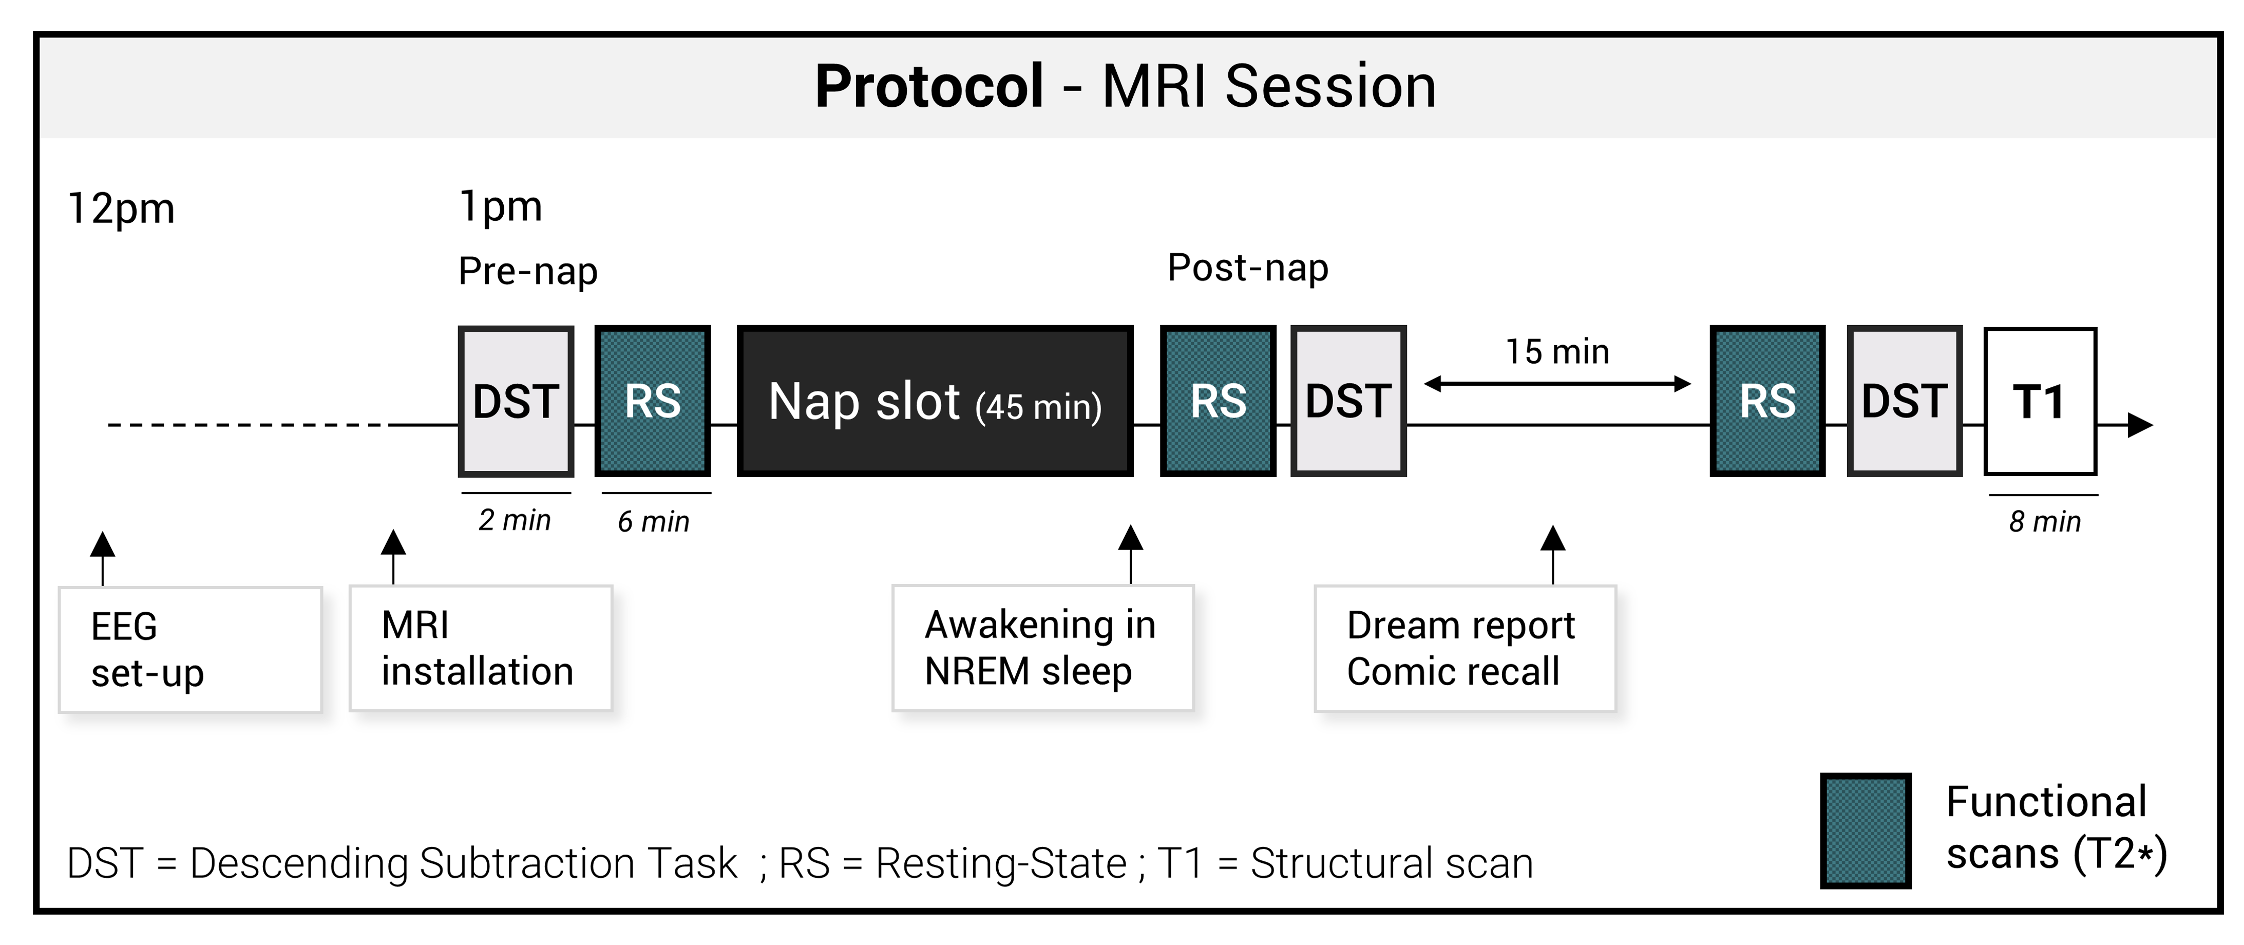
\includegraphics[width=\textwidth]{Fig/Intro/Intro_paradigm_fMRI/Intro_paradigm_fMRI.png}
	\caption[Experimental design of the fMRI study]{Experimental design of the sleep inertia fMRI study. After lunch at 11.30 am, participants were conducted to the neuroimaging center (CERMEP). During the first half hour, experimenters installed on the participant’s head a MRI compatible EEG cap. Participants were then installed in the MRI scanner. They read a 5 min cartoon during the calibration of the eye-tracking camera, and then performed a mental calculation  task (descending subtraction task, DST) for 2 minutes. The first resting-state scan was then acquired, with the instructions to remain awake and look at a central fixation cross on the screen. At the end of the scan, participants were informed that they could sleep during the next 45 min. At the end of the nap slot, participants were awakened, if they were sleeping, by calling their first name and the 2nd resting state scan was acquired. At the end of the scan, the 2nd DST was performed. During the following 10 minutes, subjects were asked about their dream(s) and sleep in the scanner and about the cartoon. Then the 3rd resting state scan and DST were performed (about 25 min after awakening). Finally, an 8-min T1 anatomical scan was acquired.Participants were selected if they reported and subsequently confirmed during a phone interview having a high or low DRF (DRF superior to 5 dream recalls per week and inferior to 2 dream recalls per month respectively) and having no sleep disturbances. Importantly, the night before the experiment, the subjects underwent a partial sleep deprivation (they were allowed to sleep between 5 am and 8 am) in order to facilitate sleep in the MRI scanner and heighten the sleep inertia effect.}
	\label{fig:intro:problematics-fmri-paradigm}
\end{figure}

\subsection{Brain networks dynamics during sleep inertia}
\label{sec:problematic:inertia:overview}

In addition with comparing the differential brain functional organization of high and low dream recallers during sleep inertia, this study offers the possibility to investigate thoroughly - by pooling the two groups - the brain networks changes across the sleep inertia period. Indeed, while the behavioral aspects of sleep inertia are well documented, only a limited amount of studies investigated its cerebral correlates until now. Using EEG, some studies have found a persistence of slow wave activity in the minutes following awakening, specifically in posterior areas, a phenomenon which has been suggested to represent the electro-physiological signature of sleep inertia \citep{ogilvie_falling_1992, ferrara_electroencephalographic_2006, marzano_recalling_2011, gorgoni_eeg_2015}. Using PET, \citet{balkin_process_2002} reported that the brain areas whose regional cerebral blood flow (rCBF) was increasing between 5 to 20 min post awakening were primarily anterior heteromodal areas (e.g. lateral prefrontal cortices, and anterior insula). They also reported shifts in the relative levels of rCBF between pairs of brain regions (orbitofrontal cortex and ventromedial caudate nucleus, dorsolateral prefrontal cortex and mesencephalic reticular formation) between 5 and 20 min post awakening, leading them to propose that recovery from sleep inertia could hinge on a resumption of normal levels of both rCBF and functional connectivity between brain areas. The latter hypothesis has been tested in two recent resting-state functional magnetic resonance imaging (fMRI) studies which investigated the variations in brain connectivity between pre-sleep wakefulness, nocturnal sleep (without previous sleep deprivation) and post-sleep
wakefulness \citep{wu_variations_2012, tsai_local_2014}. Using paired comparisons between pre- and post-sleep wakefulness, they found a decreased connectivity within the sensory-motor network at awakening but no alterations in the default mode network. This altered connectivity within the sensory-motor network is coherent with the poor motor performances observed at awakening but does not explain the impairments observed in other domains (e.g. cognitive tasks such as mental calculation, \citealp{tassi_sleep_2000, trotti_waking_2016}). Yet, some modifications of the default mode network connectivity could be expected at awakening since several neuroimaging studies showed consistent alterations of the default mode network connectivity during sleep, fatigue and/or falling asleep (see \citealp{picchioni_sleep_2013} for a review).

By looking at the brain and behavioral changes associated with sleep inertia, independently of the two group, our paradigm provides an ideal starting point to study, as wished by \citet{trotti_waking_2016} in her recent review, \q{the which and how functional brain networks are altered in the minutes following awakening}. Moreover, participants were partially sleep deprived on the night before and awakened from a 45 min mid-afternoon nap, in the deepest possible sleep stage (N3 sleep; see section \ref{sec:dream-research:sleep:stages}). Both sleep deprivation and awakening in N3 sleep have been associated with increased sleep inertia \citep{tassi_sleep_2000}. In addition with being ecological (short nights compensated by a daytime nap being common in young adults \citep{faraut_napping:_2016}, this paradigm will allow us to study sleep inertia in its most intensified form.

\subsection{Resting-state functional connectivity changes in high and low dream recallers}
\label{sec:problematic:inertia:resting-drf}

Another way to analyze the results of this study is to concatenate, for each subject, the three 6 minutes resting-state scans (i.e. pre-sleep, 5 min after awakening and 25 min after awakening, see Figure \ref{fig:intro:problematics-fmri-paradigm}). This approach allows to investigate the differences in functional connectivity, at rest, between high and low dream recallers. This analysis follows and the work of \citet{eichenlaub_resting_2014} regarding the differences in resting-state rCBF between high and low dream recallers (see section \ref{sec:dream-recall:param:neuro}). As a reminder, they have found higher rCBF, during both sleep and wakefulness, in two core regions of the default mode network (i.e. the TPJ and MPFC), which also appear to be involved in dream production and / or recall \citep{solms_neuropsychology_1997}. Our paradigm provide thus an ideal framework to further investigate the trait neurophysiological differences between HR and LR, and notably the resting-state functional connectivity within and between brain networks, which was not possible with PET. Since studies have shown that there is a tight coupling between cerebral blood flow and brain functional topology during rest \citep{liang_coupling_2013}, we expect that compared to low dream recallers, high dream recallers will have a higher functional connectivity within the default mode network, specifically between the MPFC and TPJ. If this turns out to be true, it will be an additional key argument that the brain functional organization of high and low dream recallers differs. We also hypothesize that a differential brain functional organization could reflect psychological traits factors (i.e. thinner boundaries, higher level of absorption and higher creativity in high dream recallers, see section \ref{sec:dream-recall:param:link}). To test this latter hypothesis, we have included in our paradigm several psychological tests to measure creativity, personality traits and cognitive abilities. They will be further detailed in the results section.

\section{Sleep and dream habits in French students}
\label{sec:problematic:survey}

Epidemiological investigations in healthy subjects combining questions on both sleep and dreaming are relatively rare. Such measures are yet necessary to establish and keep up to date sleep and dream norms in the general population. Of particular interest is the college population, which is more at risk of suffering from sleep difficulties than the general population \citep{buboltz_sleep_2001, curcio_sleep_2006, forquer_sleep_2008, lund_sleep_2010}.

In order to recruit participants for our above-mentioned fMRI sleep study (section \ref{sec:problematic:inertia}), we have sent an announcement to several mailing lists of students from Lyon University. The announcement comprised a link to an online questionnaire about sleep and dream habits that participants had to fill out. The analysis of the responses provided up-to-date data on sleep and dream habits of a large sample of French college students, pertaining to different academic fields (i.e. humanities, science, medicine). Because our survey included relatively rare questions (e.g. frequency of recurrent and lucid dreams, sleepwalking, sleep-talking, sleep agitation), and thanks to a large sample of students including much more males than in previous studies (i.e. more than one third), we believe that this study will make a significant contribution to the limited number of previous epidemiological studies. We do not formulate explicit assumptions related to this study, as it is mainly exploratory and descriptive.

\section{The memory sources of dream content}
\label{sec:problematic:wle}

As we mentioned earlier, there is ample evidence that waking-life experience (WLE) finds its way into dreams (which led to the so-called continuity hypothesis, \citealp{schredl_continuity_2003}). However, the characteristics and time course of the waking memory sources integrated into dreams are still unclear. We have reviewed in section \ref{sec:dream-content:sources:memory} the five factors that are positively associated with the likelihood of a WLE to be incorporated into dreams \citep{schredl_characteristics_2010}. However, these factors are not fully understood and require further clarification. This is the case for instance regarding the temporal distance between the WLE and its incorporation into dreams on one hand, and the emotional intensity of the WLE on the other hand. Indeed, it is generally admitted that there is a preferential incorporation of recent and emotional WLE into dreams \citep{botman_dream_1990, strauch_dem_2004, grenier_temporal_2005, schredl_factors_2006, malinowski_evidence_2014}. However, some characteristics of dream content do not fit with this modeling of the data. Firstly, some body injuries - be it congenital or acquired - such as amputation, paraplegia and deafness, are less incorporated into dream reports than this model would predict considering how highly emotional and central to the person’s life they are \citep{voss_waking_2011, saurat_walking_2011, bekrater-bodmann_post-amputation_2015}. Secondly, as noticed by \citet{freud_interpretation_1900} more than one century ago, dream content seems to integrate a non-negligible proportion of non-emotional and mundane day residues (i.e. WLEs from the day before the dream).

\subsection{Paradigm and predictions}
\label{sec:problematic:wle:predictions}

We believe that the results showing a preferential incorporation of emotional WLE into dreams may be partly explained by the classic method used in experimental studies so far, i.e. the content matching paradigm. It requires the participants to rate a posteriori (i.e. at the end of several days of experiment), similarities between a day diary and a dream diary completed for 14 days (e.g. \citealp{schredl_factors_2006, malinowski_evidence_2014}). Such a method has the advantage of controlling for retrospective availability of memories for elements when participants relate dream content to WLEs, but it has the drawback of missing mundane experiences that are not recorded in the day diary. As a consequence, previous studies could not fully assess whether mundane WLEs were incorporated into dreams. To fill this gap, we designed a study which aims to investigate in further details the characteristics of the WLEs incorporated into dreams, notably by assessing their remoteness on a life-time scale and by taking mundane WLEs into account. To do so, instead of asking dreamers to keep a day diary, we asked participants to report and characterize the WLEs related to their dreams immediately upon awakening. This strategy presents several advantages regarding previous methods. Firstly, any remembered WLE at any timescale can be considered. This method offers then the possibility of investigating the incorporation of WLEs across the whole life span, which has been rarely attempted until now \citep{grenier_temporal_2005, marquardt_empirical_1996}. Secondly, as the reported memory sources of a dream are dependent on the delay between the dream and the task to report memory sources, the sooner the task after the dream, the more chances we have to identify the true memory sources of the dream \citep{cavallero_dream_1987}. Thirdly, as the connections between elements of waking life and dream content are assessed when the memories of the preceding days are still fresh, this method enables the recall of trivial WLEs from at least the few days before the dream. Using this new approach, we are able to test whether emotional WLEs are still preferentially incorporated into dream reports when trivial WLEs are taken into account and to investigate the emotionality and significance of WLEs incorporated into dreams as a function of their remoteness.

We predict that this methodology would enable us to observe that a large proportion of the WLEs incorporated into dreams are mundane. Regarding the temporal remoteness of the WLEs incorporated into dreams, we expect to find not only a large contribution of the day before the dream \citep{marquardt_empirical_1996} but also a significant contribution of remote WLEs \citep{verdone_temporal_1965, grenier_temporal_2005, llewellyn_such_2013}. Finally, given previous results showing a tendency for dreams to incorporate preferentially emotional WLEs \citealp{schredl_factors_2006, malinowski_evidence_2014}, and the claim that day residues are predominantly mundane \citep{freud_interpretation_1900}, we predict an interaction between remoteness and emotionality for WLEs incorporated into dreams. Specifically, we expect that day residues would be scored as less important and less emotionally intense than would more remote WLEs incorporated into dreams.

\section{An open-source software for sleep data}
\label{sec:problematic:software}

During my PhD thesis, I have been working extensively on polysomnographic sleep recordings, notably to score sleep microstructural events (e.g. arousals, rapid eye movements; see section \ref{sec:problematic:arousals}) and sleep stages (see section \ref{sec:problematic:inertia}). While the detection of sleep microstructural events is usually done with automatic algorithms, the identification of sleep stages is traditionally done visually by an expert. For both visual sleep staging and automatic microstructural analysis, sleep researchers use either commercial or in-house softwares. In many cases, these softwares come with their own data and hypnogram file formats, and this heterogeneity can represent a substantial obstacle for sharing of algorithms and sleep data across laboratories.

% Some of the very few free and open-sources alternatives allowing scoring and to some extent analysis of sleep data are \fnurl{Phypno}{https://pypi.python.org/pypi/phypno} and \fnurl{SpiSOP}{http://www.spisop.org/}, yet they do not include graphical integration of automatic detection and are largely based on command-line options, which are hardly accessible for users with little or no programming knowledge.

% Traditionally, the scoring of sleep micro- and macro-structure is done visually and requires therefore a considerable investment of time and effort, in addition with being subject to both inter and intra-rater variability. Sleep scoring can also be done using automatic methods which have the advantage of being fast, reproducible and with generally good agreement with visual scoring \citep{berthomier_automatic_2007, lajnef_learning_2015}. Yet automatic scoring is far from being widespread and most sleep laboratories still rely on visual scoring, using either commercial softwares or in-house packages. In many cases, these softwares come with their own data and hypnogram file formats, and this heterogeneity can represent a substantial obstacle for sharing of algorithms and sleep data across laboratories or clinics. Some of the very few existing and up-to-date open sources alternatives allowing reading and scoring of sleep data are \fnurl{Phypno}{https://pypi.python.org/pypi/phypno} and \fnurl{SpiSOP}{http://www.spisop.org/}, yet they do not include graphical integration of automatic detection and are largely based on command-line options, which are hardly accessible for users with little or no programming knowledge.


In view of this, I developed, during my PhD thesis, a free and open-source software capable of reading numerous file formats, and integrating several signal processing tools and automatic detection of sleep microstructure. At first intended for my personal use, it soon extended into a fully developed and comprehensive software, thanks to a collaboration with my fellow PhD student \fnurl{Etienne Combrisson}{https://etiennecmb.github.io/}. This software was integrated into a broader neuroscientific suite named \fnurl{Visbrain}{http://visbrain.org/}, and the specific sleep module was named \textit{SLEEP}. The primary aim of \textit{SLEEP} is to provide a fast and intuitive graphical user interface (GUI) to visualize and score polysomnographic sleep recordings. In order to be widely disseminated, the software must support a large range of data file formats, both proprietary (e.g. BrainVision) and public (e.g. European Data Format). It should also be able to handle the great heterogeneity in hypnogram formats (e.g. sampling frequency of the hypnogram, values assigned to each sleep stage). Finally, to provide a significant scoring aid, the software should include several automatic detection algorithms (e.g. spindles, K-complexes, slow-waves) and several signal processing tools (e.g. filtering, referencing). Altogether, we believe that this software could represent a major methodological development in the field of sleep research.

\section{Summary}
\label{sec:problematic:summary}

\begin{figure}[htb]
	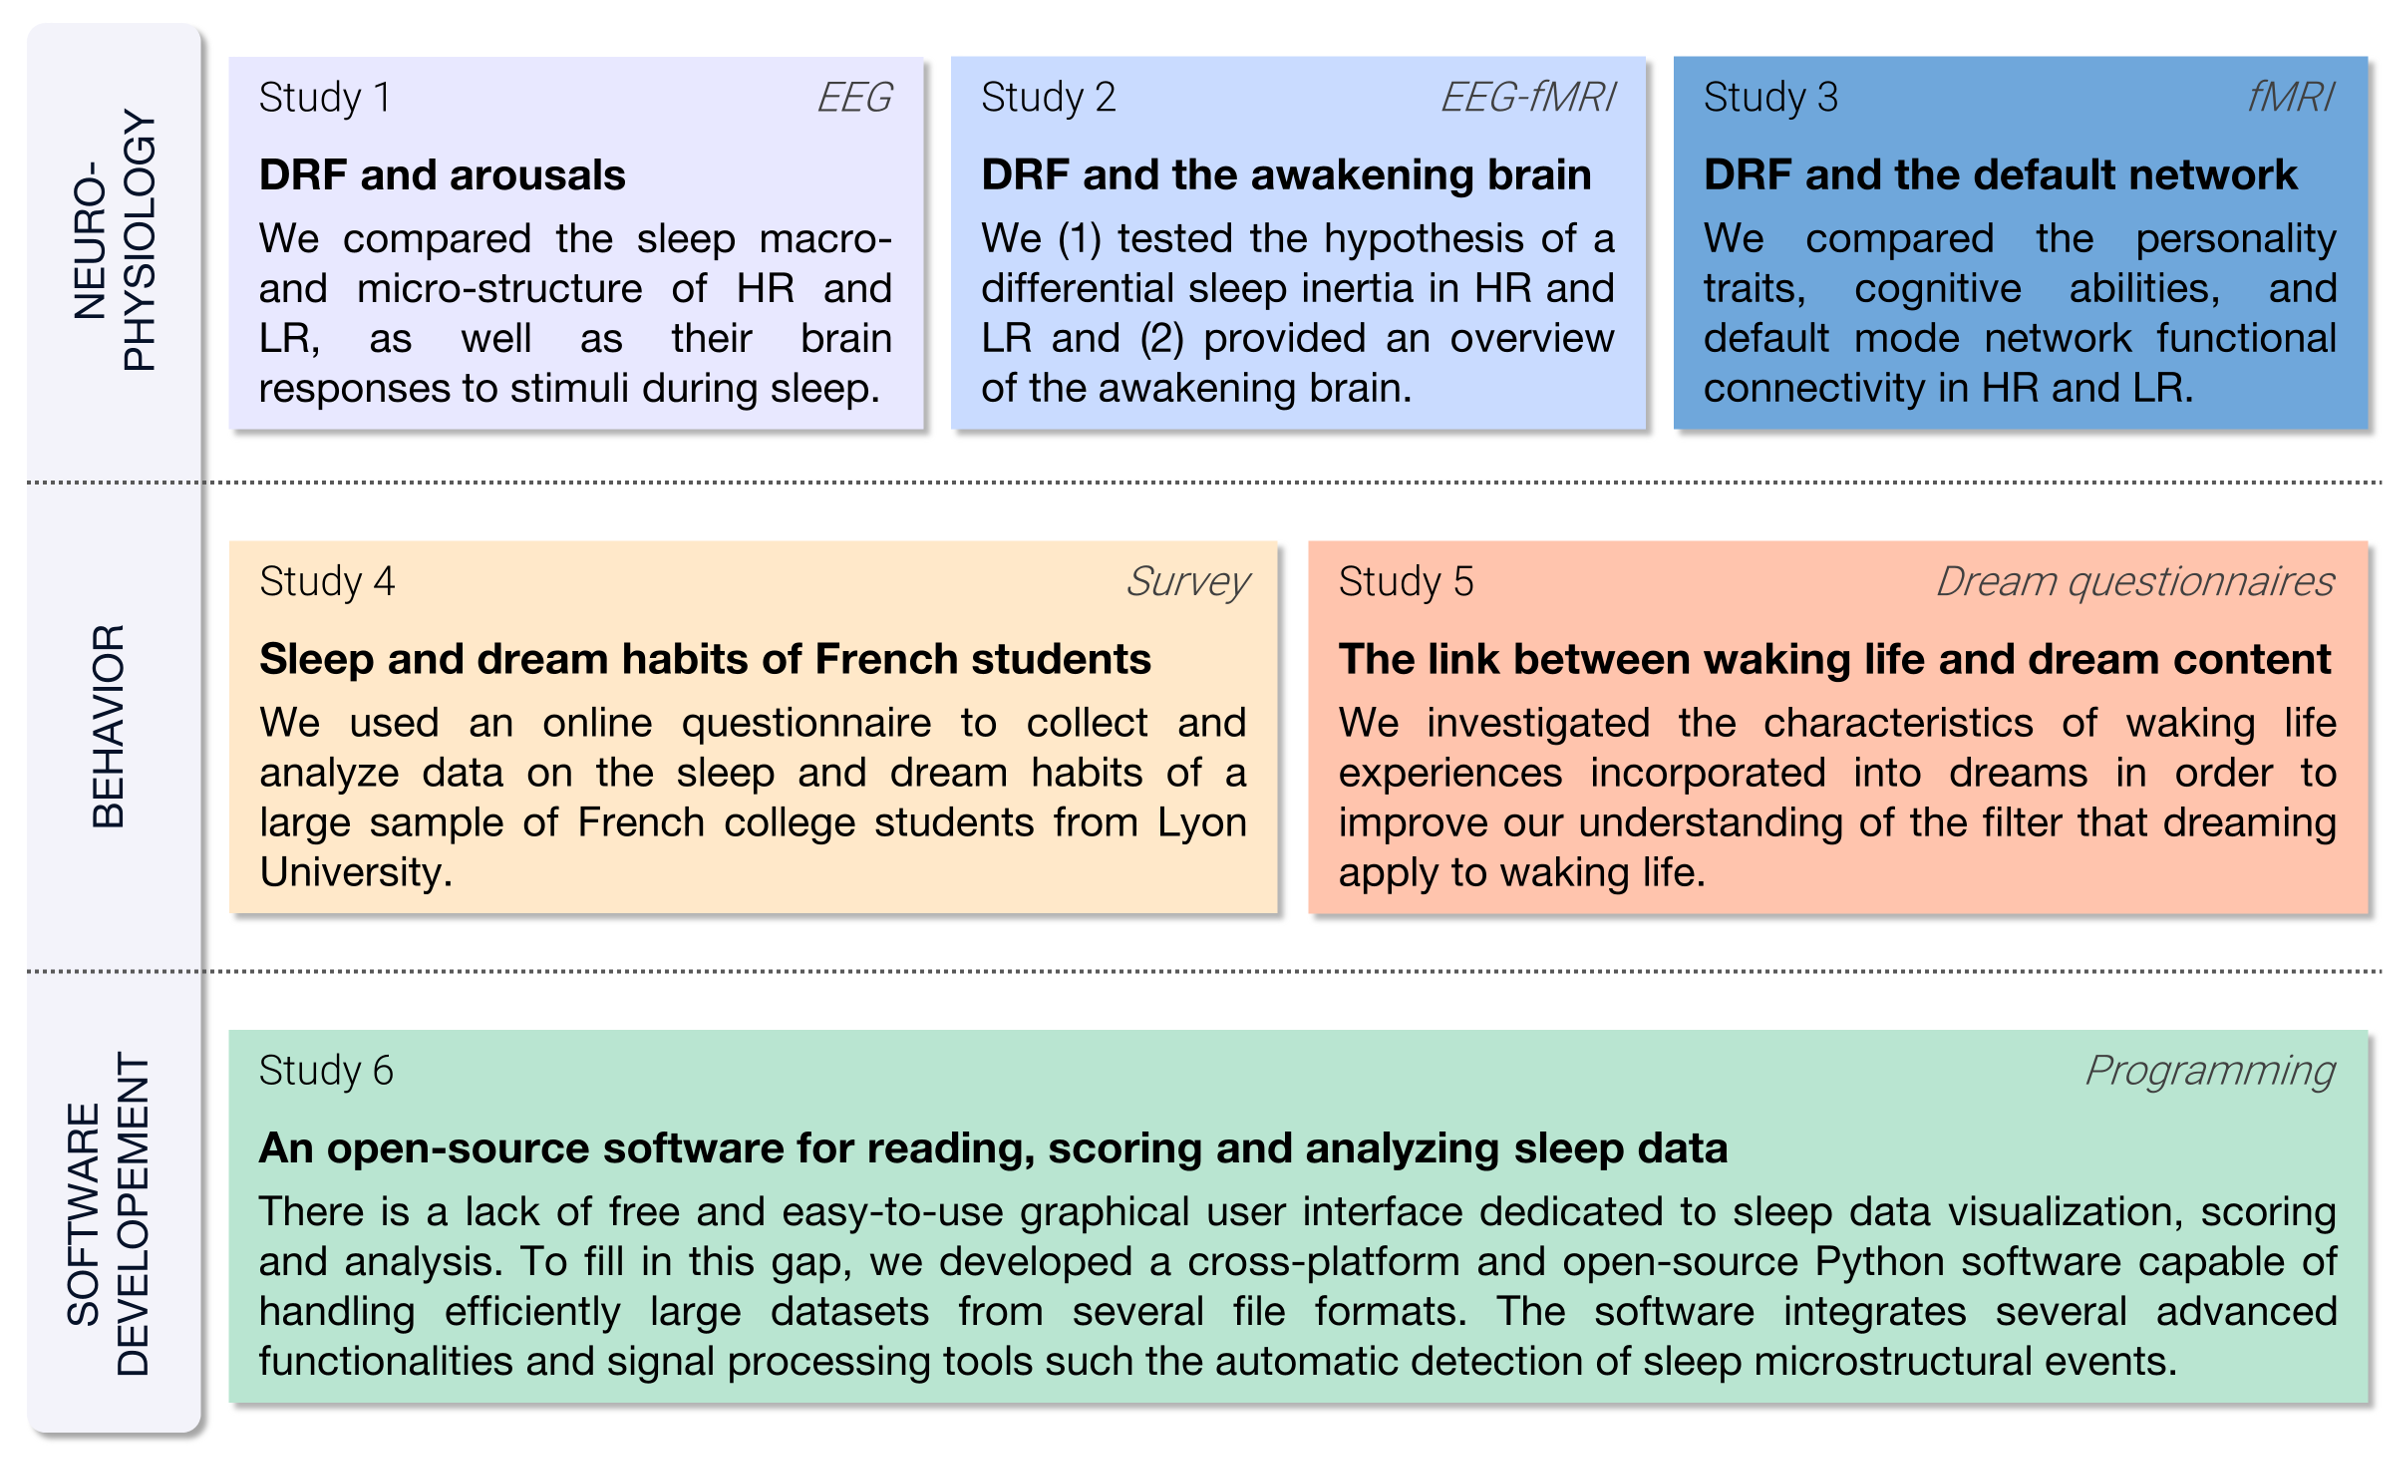
\includegraphics[width=\textwidth]{Fig/Intro/Intro_Problematics/Intro_Problematics.png}
	\caption[Summary of the studies conducted in this thesis]{Summary of the studies conducted in this thesis. In the first two studies, we investigated the neurophysiological correlates of dream recall frequency (DRF) with regards to nocturnal arousals and sleep inertia respectively. Studies 3 is an epidemiological survey of the sleep and dream habits in French college students from Lyon University. In study 4, we conducted a close analysis of the links between waking-life and dream content, with a special emphasis on the incorporation of remote and / or mundane memories. Finally, study 5 relates to the ongoing development of an open-source software to visualize, score and analyze polysomnographic sleep recordings.}
	\label{fig:intro:problematics-summary}
\end{figure}
